\documentclass[24pt, a0papper, portrait]{tikzposter}
\makeatletter
\def\title#1{\gdef\@title{\scalebox{\TP@titletextscale}{%
\begin{minipage}[t]{\linewidth}
\centering
#1
\par
\vspace{0.5em}
\end{minipage}%
}}}
\makeatother
\usepackage[utf8]{inputenc}
\usepackage{subfig}
\usepackage[retainorgcmds]{IEEEtrantools}
\graphicspath{ {./images/} }
 
\title{Simulation of Various Channelizer Structures 
       Directed by Cyclostationary Detector}
\author{Brian H. Hulette, Amir I. Zaghloul}
\institute{Virginia Tech Dept. of Electrical Engineering}
 
\usetheme{Autumn}
 
\begin{document}
 
\maketitle

\begin{columns}
\column{0.33}
\block{Introduction}
{
We present a Software-Defined Radio (SDR) system for detecting and tuning 
multiple signals of interest. The system will sample
at a high rate to acquire a large section of the frequency spectrum. Then it will attempt to
detect the frequencies within the acquired range that contain signals of
interest, and then tune, filter, decimate, and demodulate those signals. 

Detection is performed by a cyclostationary detector, which
exploits the cyclostationary properties exhibited by most digital signals with
a fixed symbol rate.  Tuning, filtering, and decimating are performed by
a configurable filter bank, so that many signals can be isolated
simultaneously.  The block diagram shown in Figure~\ref{fig:block_diagram} 
illustrates this system.

        \begin{tikzfigure}[High-level block diagram of our system. An analog front-end and
        ADC are used to bring wideband data into our Software-Defined Radio.
        There, a detector directs a configurable filter bank to isolate $N$
        signals of interest, which are then demodulated. The highlighted
        detector and filter bank are the components examined here.]
            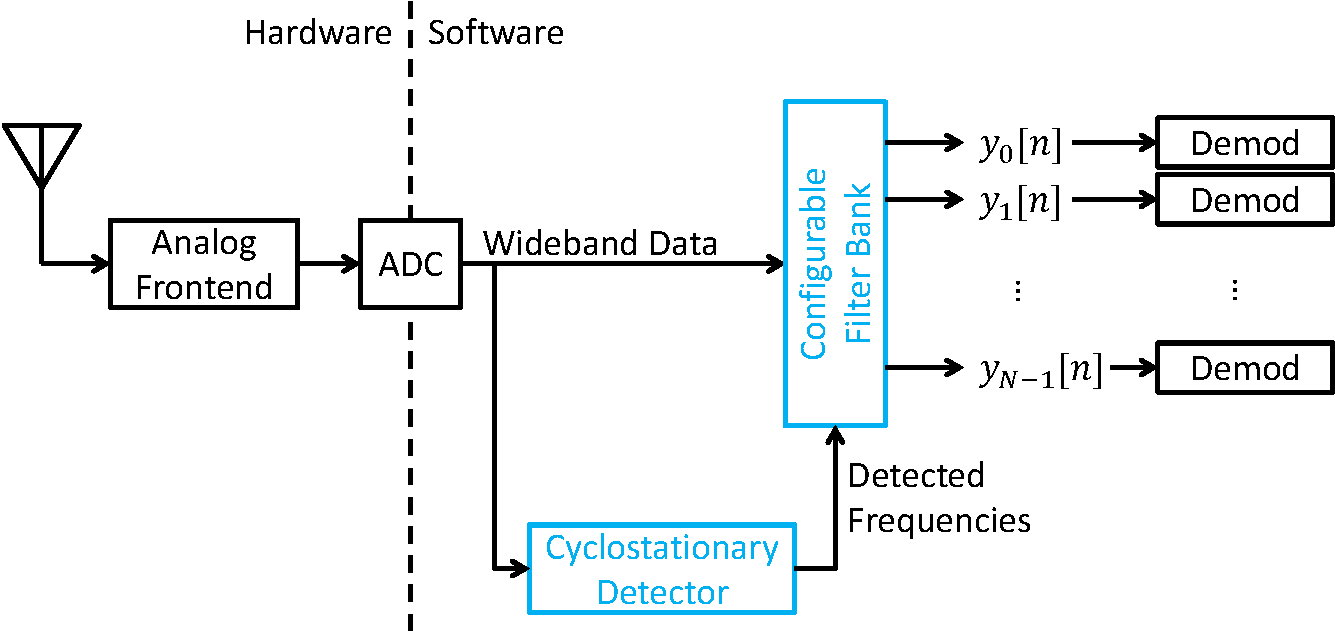
\includegraphics[width=\linewidth]{block_diagram}
            \label{fig:block_diagram}
        \end{tikzfigure}

We are primarily concerned with two components: the cyclostationary detector,
and the configurable filter bank.  Two different filter bank structures are
examined: an overlap-save filter bank, and a combined polyphase
analysis/synthesis filter bank, composed of a polyphase analysis filter bank
followed by several polyphase synthesis filter banks.  These structures are
evaluated on two important criteria:
1) Their ability to accurately reproduce every detected signal, and 2) Their
   computational efficiency when combined with a cyclostationary detector.

    }
 
    \block{Cyclostationary Detection}
    {
Often signals are modeled as stochastic random processes with properties such as
mean and variance, but many man-made signals, particularly digital communications,
can be modeled with another statistical property called
\emph{cyclostationarity}, which implies the signal has some parameter which
varies periodically with time. The frequency of this variation is called the cyclic
frequency, $\alpha$. \cite{Gardner1}.


Of particular interest for this project is second-order cyclostationarity,
where a signal has a periodic auto-correlation, $R_{xx}(t, t+\tau)$:

%\vspace{1cm}
\begin{IEEEeqnarray}{lCl}
    R_{xx}(t, t+\tau) = E\{x(t)x^*(t+\tau)\} = \sum_{\alpha} R_{xx}^{\alpha}(\tau)e^{j2 \pi \alpha t}
\end{IEEEeqnarray}
%\vspace{1cm}

The function $R_{xx}^{\alpha}(\tau)$ is the cyclic auto-correlation function (CAF), given by:

\begin{IEEEeqnarray}{lCl}
    R_{xx}^{\alpha}(\tau) = \lim_{T \to \infty} \frac{1}{T}\int_{-T/2}^{T/2} R_{xx}(t, t+\tau)e^{-j2\pi \alpha t} dt
\end{IEEEeqnarray}

Estimates of the CAF function can be used for signal detection in the time
domain. Another useful function for detection is the Fourier transform of the
CAF, called the Spectral Correlation Density (SCD), given by:

\begin{IEEEeqnarray}{lCl}
    S_{xx}(\alpha, f) = \int_{-\infty}^{\infty} R_{xx}^{\alpha}(\tau)e^{-j2\pi f \tau} d\tau
\end{IEEEeqnarray}

Estimates of the SCD can be used for detection in the frequency domain, as illustrated in Figure~\ref{fig:scd}
        \begin{tikzfigure}[SCD Estimates for three QPSK signals at 156.25, 312.5, and 625 kbaud. SCD at $\alpha = 0$ Hz is equivalent to PSD, SCD at $\alpha=625$ Hz highlights signal at that baud rate.]
        \begin{minipage}[b]{0.45\linewidth}
            \centering
            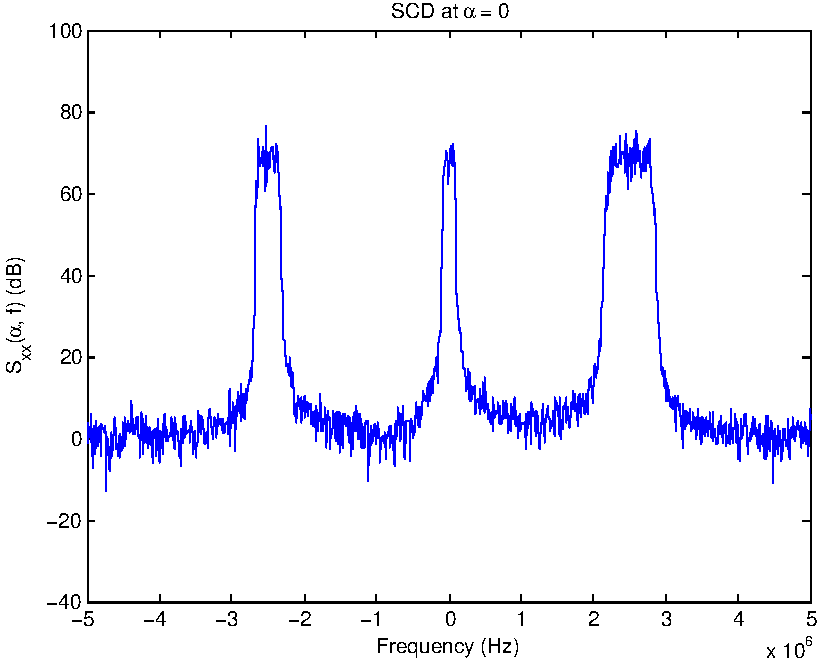
\includegraphics[width=\textwidth]{cyclo_0}
        \end{minipage}
        %\hspace{0.5cm}
        %\begin{minipage}[b]{0.45\linewidth}
        %    \centering
        %    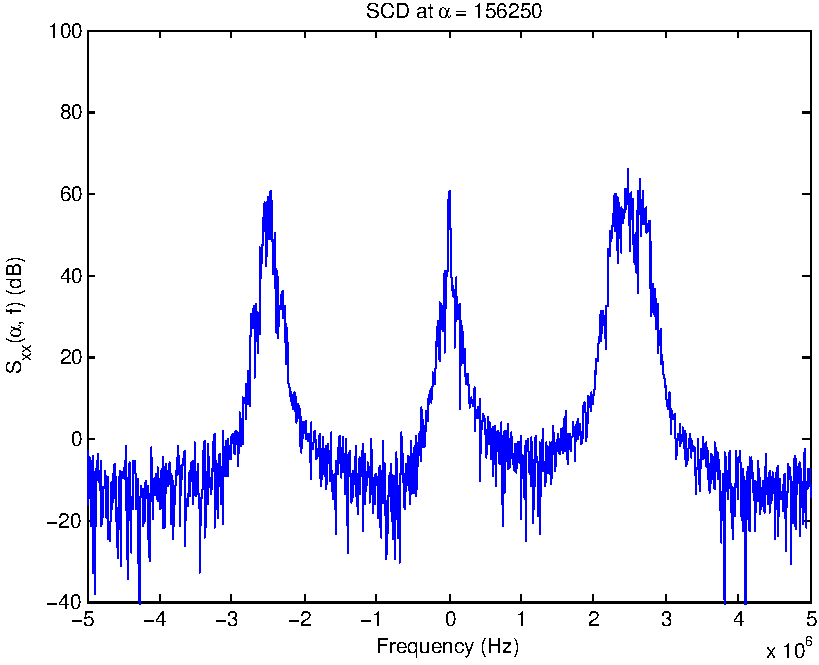
\includegraphics[width=\textwidth]{cyclo_156250}
        %    \label{fig:figure2}
        %\end{minipage}
        %\begin{minipage}[b]{0.45\linewidth}
        %    \centering
        %    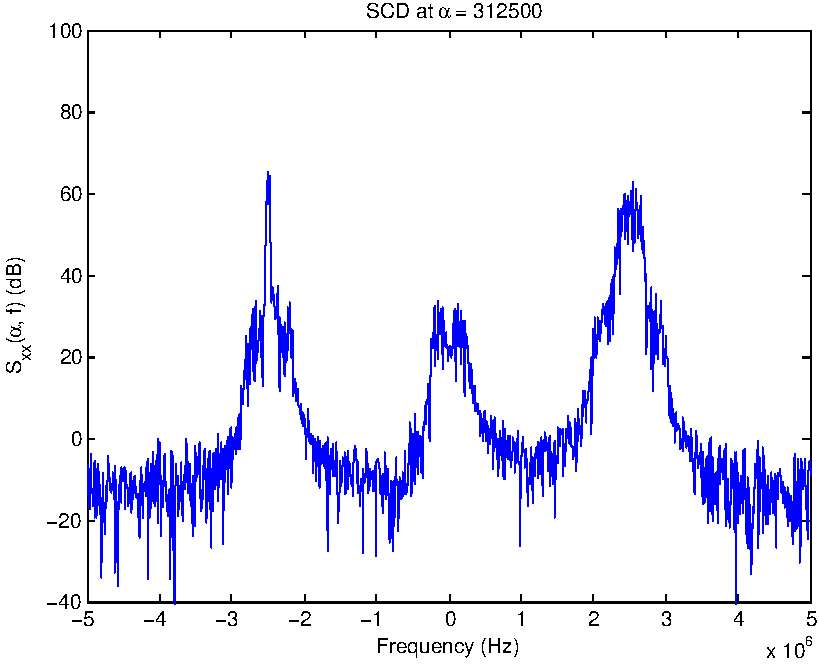
\includegraphics[width=\textwidth]{cyclo_312500}
        %    \label{fig:figure1}
        %\end{minipage}
        \hspace{0.5cm}
        \begin{minipage}[b]{0.45\linewidth}
            \centering
            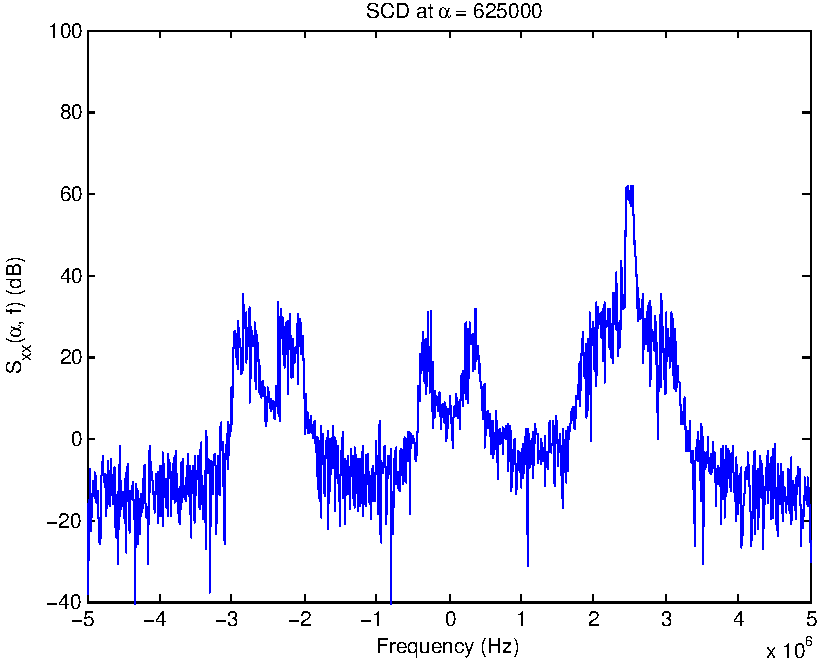
\includegraphics[width=\textwidth]{cyclo_625000}
        \end{minipage}
        \label{fig:scd}
        \end{tikzfigure}
    }
    \column{0.33}
    \block{Polyphase Filter Bank}
    {
        \begin{tikzfigure}[Non-maximally decimated ($D=M/2$) polyphase analysis and synthesis channelizers]
        \begin{minipage}[b]{0.45\linewidth}
            \centering
            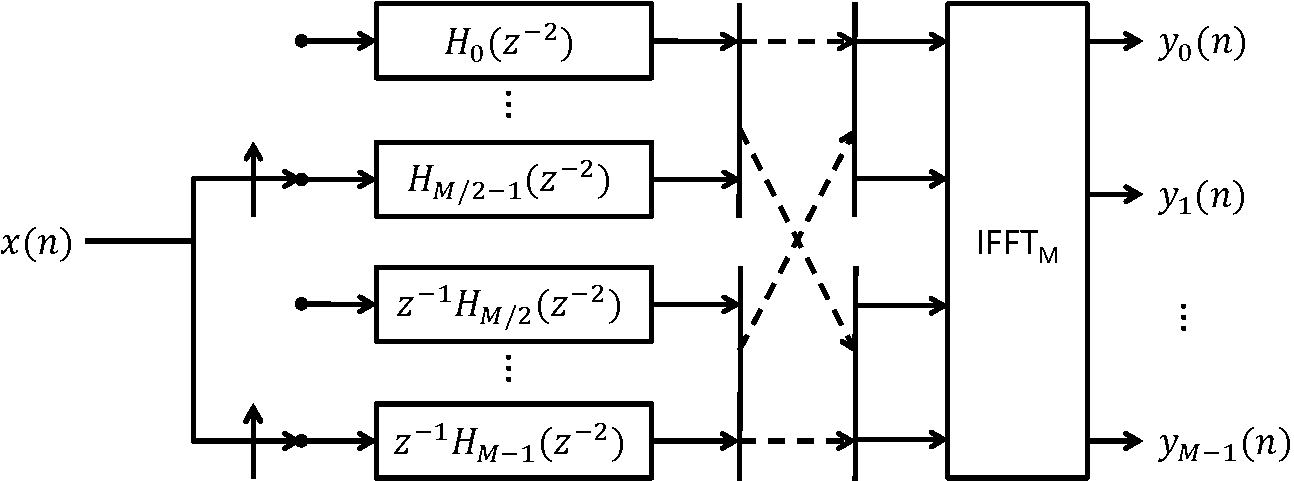
\includegraphics[width=\textwidth]{polyphase_analysis_nmdfb}
        \end{minipage}
        \hspace{0.5cm}
        \begin{minipage}[b]{0.45\linewidth}
            \centering
            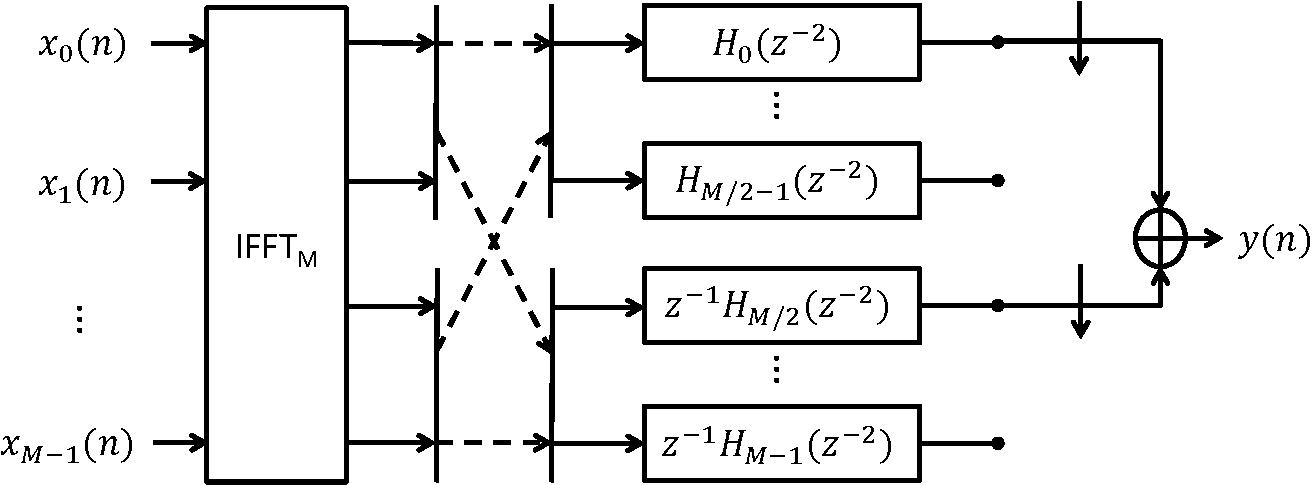
\includegraphics[width=\textwidth]{polyphase_synthesis_nmdfb}
        \end{minipage}
        \label{fig:scd}
        \end{tikzfigure}

        \begin{tikzfigure}[Using polyphase analysis and synthesis channelizers together to create a highly configurable and efficient filter bank.]
            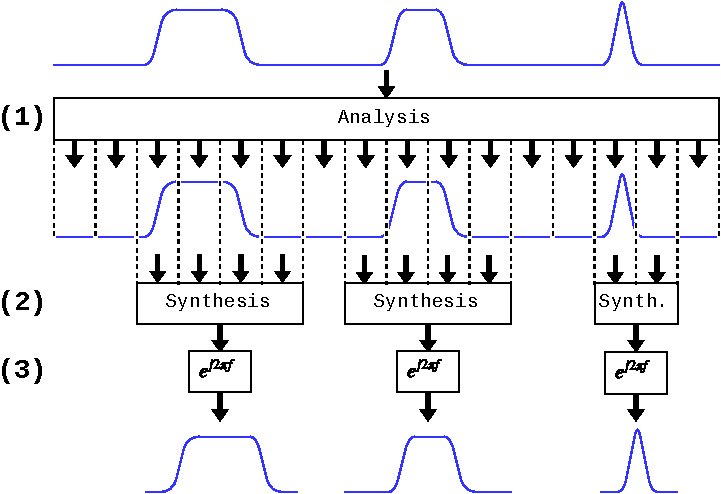
\includegraphics[width=\linewidth]{polyphase}
        \end{tikzfigure}

    }
    \block{Overlap-Save Filter Bank}
    {
        \begin{tikzfigure}[Using polyphase analysis and synthesis channelizers together to create a highly configurable and efficient filter bank.]
            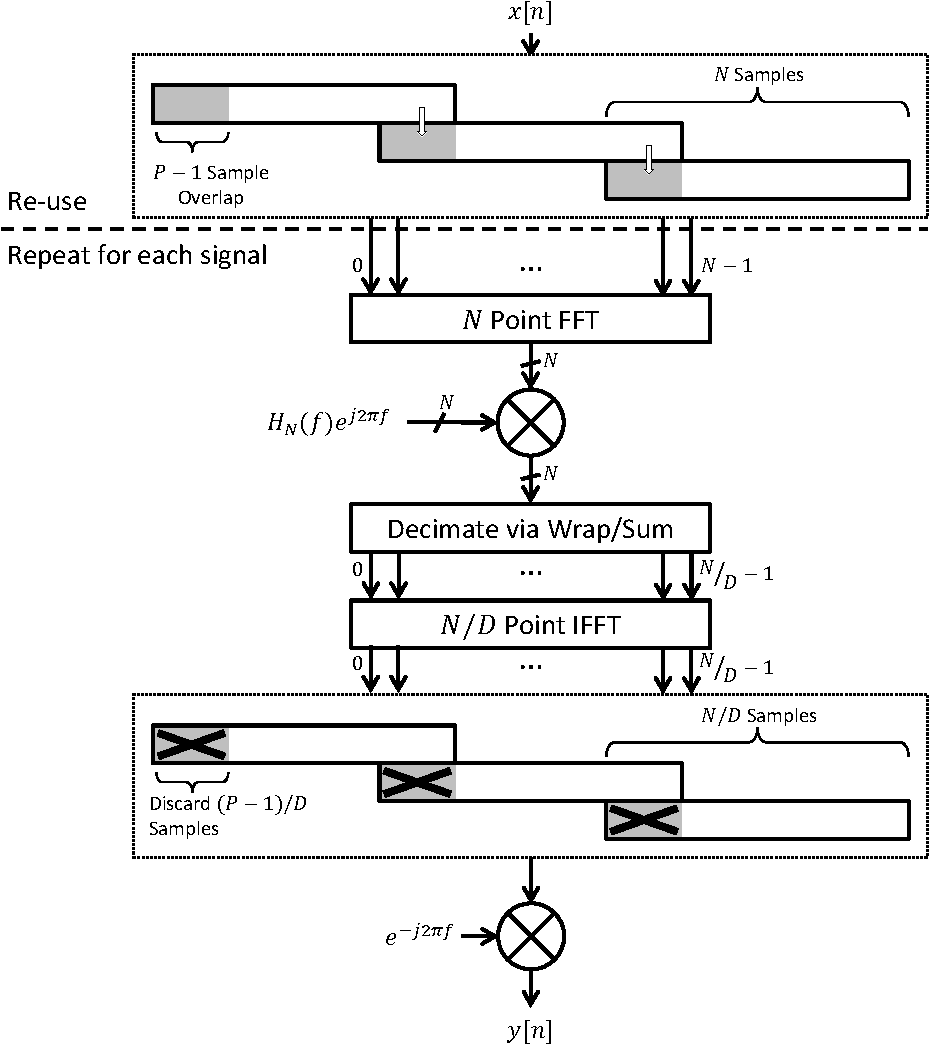
\includegraphics[width=\linewidth]{overlap_save_time_domain}
        \end{tikzfigure}
    }
    \column{0.33}
    \block{Simulation Results}
    {
        \begin{tikzfigure}[SCD Estimates for three signals at 156.25, 312.5, and 625 kbaud. SCD at $\alpha = 0$ equivalent to PSD.]
            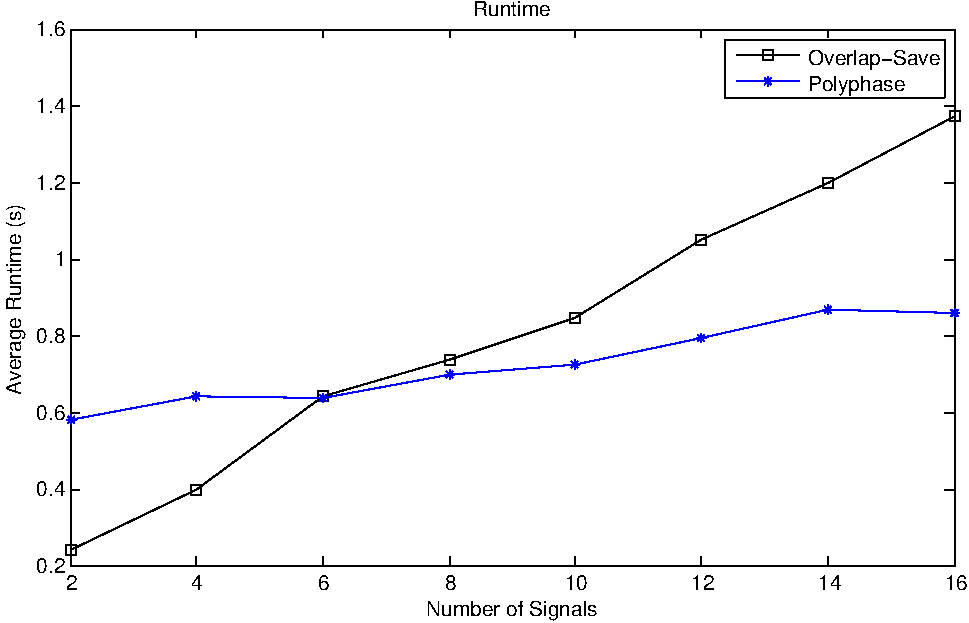
\includegraphics[width=\linewidth]{runtime_comparison_250}
        \end{tikzfigure}
        \begin{tikzfigure}[SCD Estimates for three signals at 156.25, 312.5, and 625 kbaud. SCD at $\alpha = 0$ equivalent to PSD.]
            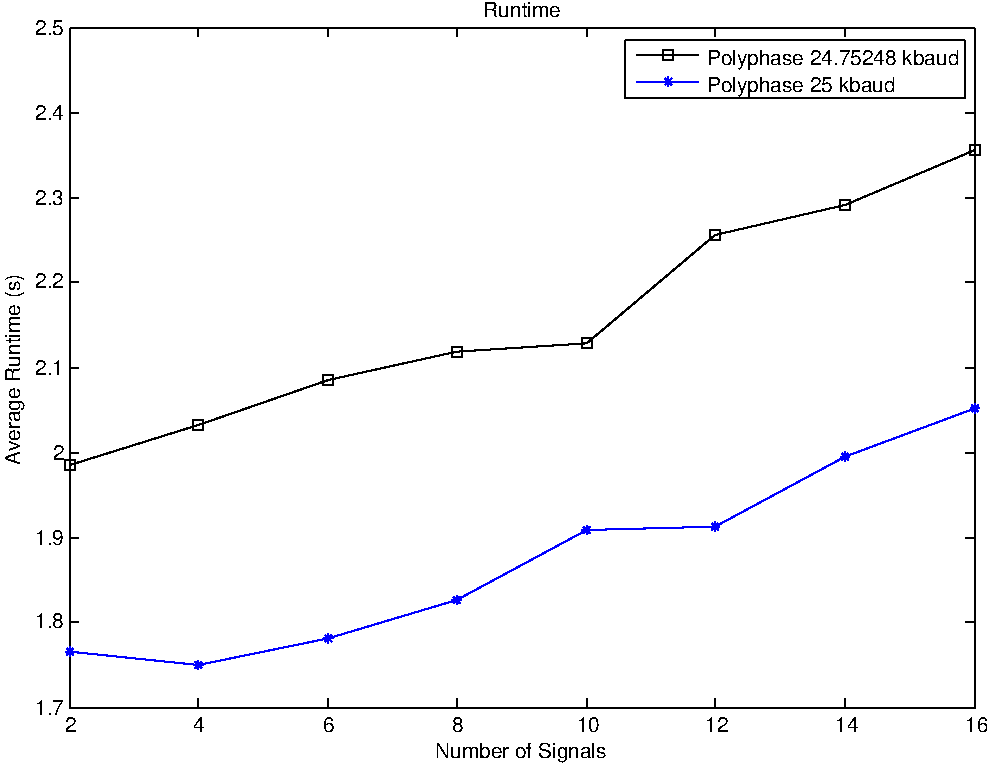
\includegraphics[width=\linewidth]{fft_runtime_comparison}
        \end{tikzfigure}
    }
\end{columns}
 
 
\end{document}
 
\end{document}
